%% ---------------------------------------------------------------------
\section{Experiments}\label{sec:experiments}

\paragraph{Setup.} Formulas are generated by \texttt{gencnf.py} and solved
with Kissat \cite{Kissat20} (default configuration unless stated) or, for
incremental runs, with CaDiCaL~1.9.5 through PySAT \cite{PySAT18}. Every
model is decoded into a rule table and re-simulated by the independent
checker \texttt{fsspcheck.c}, which reports the first length (if any) that
is not synchronized in minimal time. All timings are single-core wall-clock
times on a cloud virtual CPU.

\subsection{Calibration: four and six states}

\begin{table}[t]
\centering\small
\begin{tabular}{@{}p{0.47\textwidth}p{0.33\textwidth}r@{}}
\toprule
instance & result & time\\
\midrule
$\mathrm{MT}_4(\{2,\dots,8\};14)$ & SAT (27 partial rules) & $1.7$\,s\\
$\mathrm{MT}_4(\{2,\dots,9\};16)$ & UNSAT & $24.7$\,s\\
$\mathrm{MT}_4(\{2,\dots,10\};18)$ & UNSAT & $26.8$\,s\\
$\mathrm{MT}_4(\{2,\dots,7\};78,40)$ + links & SAT (model fails at $n=8$) & $27.5$\,s\\
$\mathrm{MT}_4(\{2,\dots,8\};78)$, lazy & UNSAT & $46.6$\,s\\
\midrule
Mazoyer's rule and $\mathrm{MT}_6(\{3,\dots,12\};78,40)$ + links & SAT (as required) & ---\\
$\mathrm{MT}_6(\{2,\dots,12\};78,40)$ & SAT, model fails at $n=13$ & $534$\,s\\
\bottomrule
\end{tabular}
\caption{Calibration. $\mathrm{MT}_k(\mathcal N;M,N')$: lengths $\mathcal N$,
half-line up to anti-diagonal $M$, pumping pairs up to $N'$ (omitted when not
used).}\label{tab:calibration}
\end{table}

For four states our encoding reproduces the theorem of Balzer and Sanders
within half a minute (\cref{tab:calibration}): the formula for the lengths
$2,\dots,9$ is unsatisfiable, whereas $27$ partial rules (counted on the
transitions they actually use, by an independent depth-first enumeration
exploring $1.09\cdot10^8$ nodes) synchronize all lengths $2,\dots,8$.
Extending the half-line to anti-diagonal $78$ already rules out lengths
$2,\dots,8$. Note that we do not assume $\delta(\ast,\mathsf L,\mathsf L)=
\mathsf L$, so this is a slight strengthening of the four-state result.

For six states the solver finds models as well, but, instructively, the
first model found for the lengths $2,\dots,12$ is not a solution: it fails at
$n=13$ although millions of genuine six-state solutions exist
\cite{NguyenMaignan20}. This ``lucky rule'' phenomenon dominates the
five-state landscape.

\subsection{Five states: the landscape of lucky rules}

\Cref{tab:five} summarizes the five-state instances solved so far. Two kinds
of lucky rules appear. Rules of the first kind have a \emph{periodic}
half-line behind the front (\cref{fig:diagrams}(b)); they satisfy a long
line such as $n=20$ by accident but violate the pumping constraints
massively (155 violated pairs $4\le n<n'\le40$ for the rule shown). Rules of
the second kind have a chaotic half-line that eventually fires. Once the
half-line is extended and the pumping constraints are added, the solver is
forced to produce half-lines with a genuine slow boundary: in every model we
inspected, a region delimited by a line of slope $1/3$ appears
(\cref{fig:diagrams}(c)), exactly as predicted by \cref{thm:third}. The
reflected triangles of these rules, however, synchronize only the lengths
that were encoded.

\begin{table}[t]
\centering\small
\begin{tabular}{@{}lll@{}}
\toprule
instance ($k=5$) & result & time\\
\midrule
$\mathrm{MT}_5(\{2,\dots,10\};18)$ & SAT, fails at $n=11$ & $10.8$\,s\\
$\mathrm{MT}_5(\{2,\dots,12\};22)$ & SAT, fails at $n=13$ & $\approx 20$\,min\\
$\mathrm{MT}_5(\{2,\dots,9,16\};30)$ & SAT, fails at $n=10$ & $23.6$\,s\\
$\mathrm{MT}_5(\{2,\dots,9,20\};38)$ & SAT, fails at $n=10$ & $82.4$\,s\\
$\mathrm{MT}_5(\{2,\dots,8\};78,40)$ & SAT, fails at $n=9$ & $68.7$\,s\\
$\mathrm{MT}_5(\{2,\dots,10\};78,40)$ & SAT, fails at $n=11$ & $755.6$\,s\\
$\mathrm{MT}_5(\{2,\dots,11\};78)$, lazy & SAT, fails at $n=12$ & $773.9$\,s\\
\bottomrule
\end{tabular}
\caption{Five-state instances (notation as in \cref{tab:calibration}).}
\label{tab:five}
\end{table}

\begin{figure}[t]
\centering
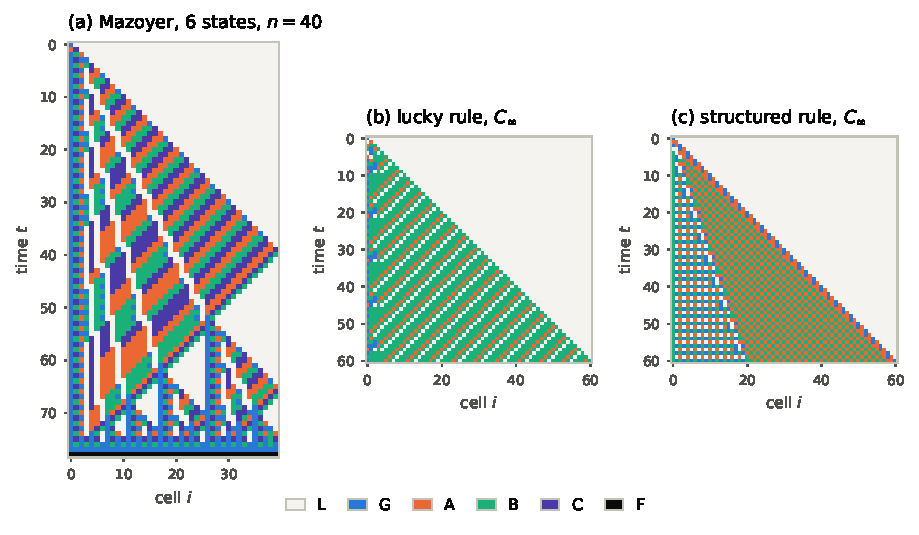
\includegraphics[width=\textwidth]{fig_diagrams.pdf}
\caption{Space-time diagrams (time downwards). (a) Mazoyer's six-state
solution on $n=40$ cells; the last row is the firing row. (b) Half-line of a
five-state rule that synchronizes the lengths $2,\dots,9$ and $20$ but
violates the pumping lemma: its background is periodic. (c) Half-line of a
five-state rule found under the pumping constraints: the boundary between
the checkered region and the diagonal background has slope $1/3$.}
\label{fig:diagrams}
\end{figure}
